\chapter{Implementacja aplikacji}
%
\section{Architektura aplikacji webowej}
Aplikacja składa się z następujących elementów (rys. \ref{fig:systemarchitecturediagram}):
\begin{itemize}
\item Mongodb - baza danych;
\item Redis \cite{redis} - przechowywanie JWT (ang. \textit{JSON Web Token}) \cite{jwt} tokenów po wylogowaniu;
\item Go - część serwerowa napisana w języku Go;
\item Android - aplikacja mobilna;
\item Docker - kontener dla wdrożenia aplikacji webowej;
\end{itemize}
\begin{figure}[ht]
\centering
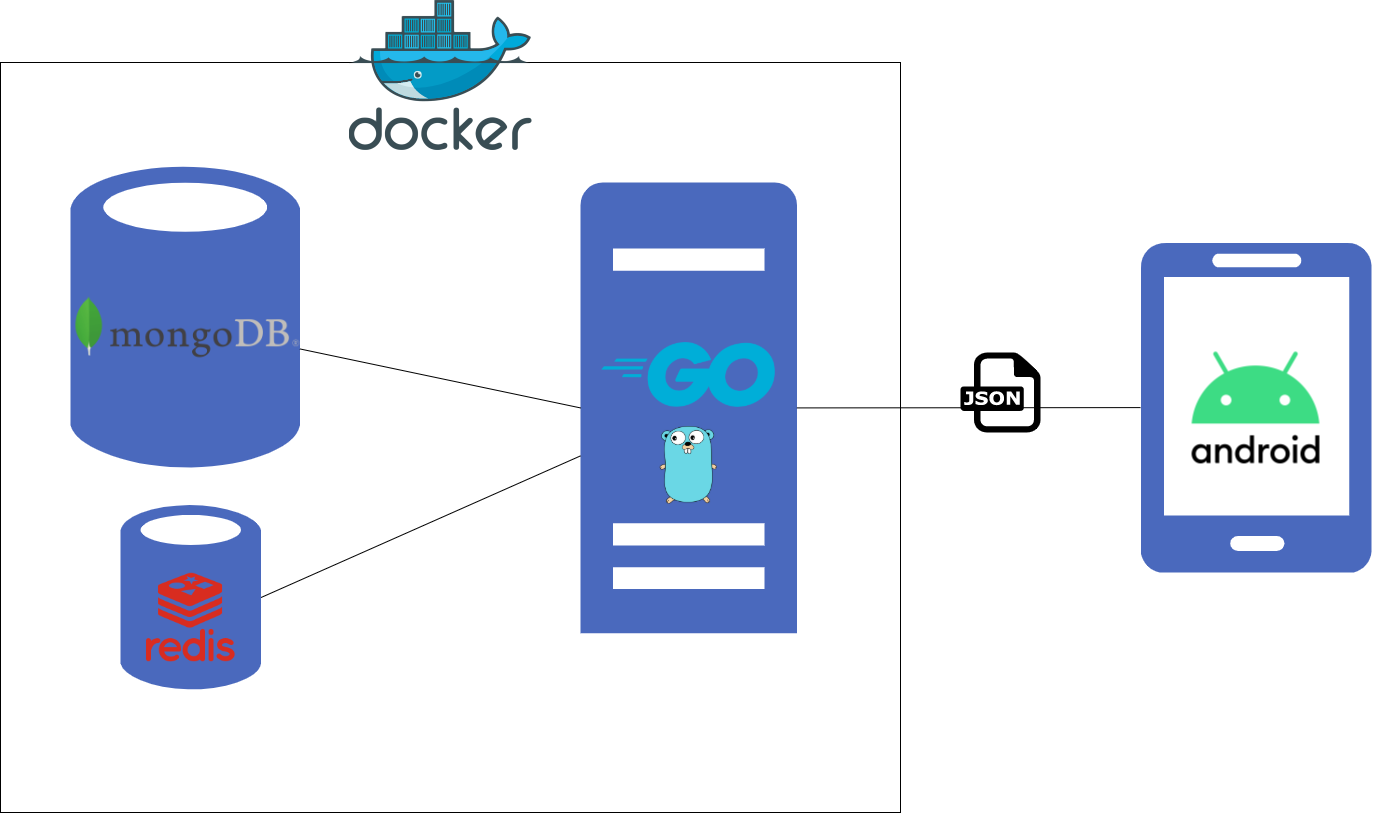
\includegraphics[width=0.8\linewidth]{rys03/system_architecture_diagram.png}
\caption{architektura systemu \cite{diagrams_net}}
\label{fig:systemarchitecturediagram}
\end{figure}
\section{Model bazy danych}
W systemie wykorzystano dwie nierelacyjne bazy danych: Mongodb i Redis.
Mongodb jest przeznaczona do przechowywania danych aplikacji.
Redis wykorzystuje się tylko do czasowego przechowywania tokenów.

\paragraph{Mongodb}

Baza danych składa się z dwóch kolekcji: ,,station'' i ,,user''.
\newline
Kolekcja ,,\textit{user}'' składa się z następujących pól:
\textit{
\begin{itemize}
    \item \_id : ObjectId(String)
    \item user\_name : String
    \item email : String
    \item password : String
    \item Model : Object :
    \begin{itemize}
        \item create\_at : ISODate
        \item update\_at : ISODate
        \item delete\_at : ISODate
    \end{itemize}
\end{itemize}
\newline
}
\newline
Przykład encji:
\begin{lstlisting}[basicstyle=\tiny\ttfamily]
    {
        "_id":ObjectId("5fb93e4b721953b7c60983c6"),
        "user_name":"newtest",
        "email":"newtest@test.test",
        "password":"$2a$04$o0WfZvdk4WUpsct.BH3zw.3MFJFmUuLe8VjJx2OeyxtZuBliMOrl.",
        "model":{
            "create_at":ISODate("2020-11-21T16:20:27.044Z"),
            "update_at":ISODate("2020-11-21T16:20:27.044Z")
        }
    }
\end{lstlisting}

Kolekcja ,,\textit{station}'' składa się z następujących pól:
\textit{
\begin{itemize}
    \item \_id : String
    \item station\_name : String
    \item owner\_id : String
    \item rating : Double
    \item latitude : Double
    \item longitude : Double
    \item description : String
    \item comments : Array :
    \begin{itemize}
        \item \_id : String
        \item user\_id : String
        \item user\_name : String
        \item text : String
        \item rating : Double
        \item model : Object :
        \begin{itemize}
            \item create\_at : ISODate
            \item update\_at : ISODate
            \item delete\_at : ISODate
        \end{itemize}
    \end{itemize}
    \item model : Object :
    \begin{itemize}
        \item create\_at : ISODate
        \item update\_at : ISODate
        \item delete\_at : ISODate
    \end{itemize}
\end{itemize}
}
\newline
Przykład encji:
\begin{lstlisting}[basicstyle=\tiny\ttfamily]
    {
        "_id":ObjectId("5fca6f81bb37f04ad438c1a5"),
        "station_name":"Station Name",
        "owner_id":"5fb828babe10c57ba70d49cd",
        "rating":3.6666666666666665,
        "description":"description",
        "latitude":57.12662933894774,
        "longitude":14.208925142884254,
        "model":{
            "create_at":ISODate("2020-12-04T17:18:57Z"),
            "update_at":ISODate("2020-12-04T17:20:55Z")
        },
        "comments":[
            {
                "_id":"5fca6ff7bb37f04ad438c1a8",
                "user_id":"5fb828babe10c57ba70d49cd",
                "user_name":"test",
                "text":"  Comment 3",
                "rating":5,
                "model":{
                    "create_at":ISODate("2020-12-04T17:20:55Z"),
                    "update_at":ISODate("2020-12-04T17:20:55Z")
                }
            },
            {
                "_id":"5fca6fe5bb37f04ad438c1a7",
                "user_id":"5fb828babe10c57ba70d49cd",
                "user_name":"test",
                "text":" Comment 2",
                "rating":3,
                "model":{
                    "create_at":ISODate("2020-12-04T17:20:37Z"),
                    "update_at":ISODate("2020-12-04T17:20:37Z")
                }
            },
            {
                "_id":"5fca6fb8bb37f04ad438c1a6",
                "user_id":"5fb828babe10c57ba70d49cd",
                "user_name":"test",
                "text":"Comment 1",
                "rating":3,
                "model":{
                    "create_at":ISODate("2020-12-04T17:19:52Z"),
                    "update_at":ISODate("2020-12-04T17:19:52Z")
                }
            }
        ]
    }
\end{lstlisting}

\paragraph{Redis}
\newline
Baza danych Redis wykorzystana tylko dla przechowywania tokenów użytkowników, które już wylogowane, ponieważ jedną z wad JWT tokenów jest to, że wygenerowany token nie można zrobić nieważny, dopóki nie skończy się czas jego działania.
Redis częściowo eliminuje ten problem.

W nim przechowuje się para klucz - wartość, pewny czas. Po upływie tego czasu zapis automatycznie jest usuwany.
Dla szybkiego wyszukiwania encja wygląda w następujący sposób: \textit{token}, \textit{token}. To pozwala często wylogować użytkowniku, ale zajmuje więcej miejsca niż encja typu: ,,\textit{user\_id}'', \textit{token}.

\section{Implementacja części serwerowej}
\subsection{Struktura RestApi}
\subsubsection{Narzędzia i technologie}
Do stworzenia serwerowej części aplikacji użyto następujących technologii:
\begin{itemize}
\item Visual Studio Code - środowisko programistyczne;
\item Go - język programowania;
\item Go Modules - system zarządzania zależnościami;
\item gorilla/mux - Router mapuje przychodzące żądania na listę zarejestrowanych tras i wywołuje moduł obsługi tego żądania, który odpowiada URL (ang. \textit{Uniform Resource Locator}) adresowi;
\item sirupsen/logrus - rejestrator strukturalny;
\item mongo-driver - sterowanie Mongodb z języka Go;
\item go-redis/redis - sterowanie Redis z języka Go;
\item dgrijalva/jwt-go - realizacja JWT w języku Go;
\item go-ozzo/ozzo-validation - pakiet wspomagający na walidację danych;
\item yaml.v2 - implementuje obsługę YAML (ang. \textit{Yet Another Markup Language});
\item google/uuid - sprawdza i generuje UUID (ang. \textit{universally unique identifier});
\end{itemize}

\subsubsection{Struktura plików RestApi}
Na rysunku \ref{fig:backend_file_structure} została przedstawiona struktura plików części serwerowej. Obok plików, niezbędnych do działania aplikacji, znajdują się pliki pozwalające na prowadzenie testów jednostkowych. Te pliki mają nazwę w postaci ,,*\_test.go''.
\begin{figure}[ht]
\centering
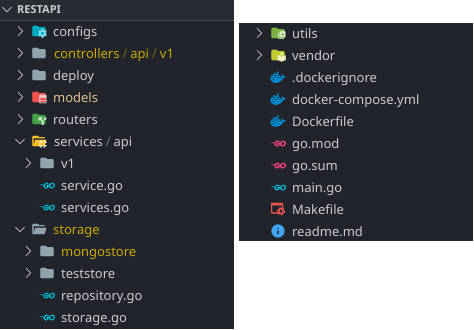
\includegraphics[width=0.25\linewidth]{rys03/backend_file_structure.png}
\caption{Struktura plików}
\label{fig:backend_file_structure}
\end{figure}
\newpage
Katalog ,,config'' zawiera pliki konfiguracyjne.
W katalogu ,,controllers'' (rys. \ref{fig:controllers}) znajdują się kontrolery, które są wykorzystywanie do połączenia poziomu serwisów z punktami końcowymi serwera (dalej Endpoint)\textbt{???}.
\begin{figure}[ht]
\centering
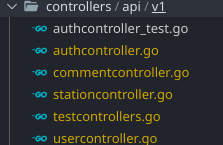
\includegraphics[width=0.25\linewidth]{rys03/controllers.png}
\caption{Struktura plików: kontrolery}
\label{fig:controllers}
\end{figure}

Do katalogu ,,deploy'' jest kompilowana aplikacja przy uruchomieniu ,,Makefile''.

Katalog ,,models''(rys. \ref{fig:model}) zawiera modeli danych do przechowywania w bazie danych oraz do przekazania do interfejsu użytkownika.
\begin{figure}[ht]
\centering
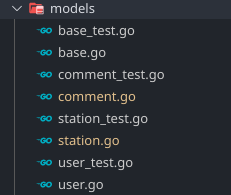
\includegraphics[width=0.25\linewidth]{rys03/model.png}
\caption{Struktura plików: modeli danych}
\label{fig:model}
\end{figure}

Katalog ,,routers'' (rys. \ref{fig:routers}) zawiera plik, w którym zachodzi mapowanie punktów końcowych z kontrolerami.
\begin{figure}[ht]
\centering
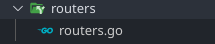
\includegraphics[width=0.25\linewidth]{rys03/routers.png}
\caption{Struktura plików: routery}
\label{fig:routers}
\end{figure}

Funkcje lub metody przechowywane w katalogu ,,services'' (rys. \ref{fig:services}) prowadzą obróbkę danych i podejmują decyzję co z nimi trzeba zrobić.
\begin{figure}[ht]
    \centering
        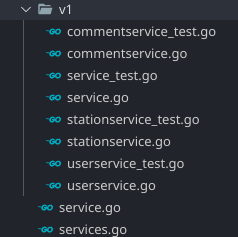
\includegraphics[width=0.25\linewidth]{rys03/services.png}
        \caption{Struktura plików: serwisy}
    \label{fig:services}
\end{figure}

Współpraca z bazą danych zachdzi w katalogu ,,storage'' (rys. \ref{fig:storage}). Katalog ,,mongostore'' wspódziałuje z Mongodb, notomiast ,,teststore'' wykorzystuje się do testowania, które będzie omówione w odpowiednim rozdiale \ref{ch:Testy}.
\begin{figure}[ht]
    \centering
        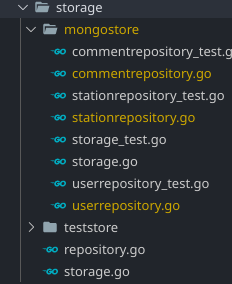
\includegraphics[width=0.25\linewidth]{rys03/storage.png}
        \caption{Struktura plików: bazy danych}
    \label{fig:storage}
\end{figure}

W katalogu ,,utils'' (rys. \ref{fig:utils}) znajdują się rzeczy wspomagające, naprykład lista błedów lub rejestracja działania serwera.
\begin{figure}[ht]
    \centering
        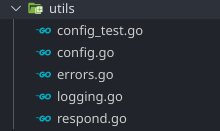
\includegraphics[width=0.25\linewidth]{rys03/utils.png}
        \caption{Struktura plików: narzędzia}
    \label{fig:utils}
\end{figure}

\subsubsection{Przepływ danych}
Na rysunku \ref{fig:backend_data_flow} został przedstawiony schemat przetwarzania i przepływu danych przy wysyłaniu zapytania do części serwerowej niniejszej aplikacji.
\begin{figure}[ht]
\centering
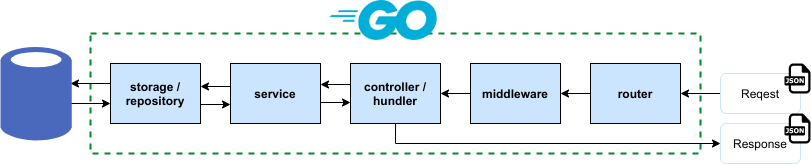
\includegraphics[width=0.9\linewidth]{rys03/backend_data_flow.png}
\caption{Przepływ danych}
\label{fig:backend_data_flow}
\end{figure}

\subsubsection{Punkty końcowe}
Część serwerowa jest napisana zgodnie z modelem Rest API. Wymiana danymi zachodzi za pomocą standardów: HTTP (ang. \textit{HyperText Transfer Protocol}), URL, JSON.
W tabeli \ref{tab:endpoints} przedstawiony spis endpointów razem z metodą ich wysłania oraz krótkim opisem.
\begin{table}[htb] \small
    \caption{Lista Enpointów części serwerowej}
    \label{tab:endpoints}
    \begin{tabular}{| m{0.5cm} | m{2cm} | m{6cm} | m{6cm} |}
    \hline
    № & Metoda & Endpoint & Opis \\
    \hline
    1 & GET & /api/v1 & Endpoint do testowania działania serwera. \\
    \hline
    2 & POST & /api/v1/login & Zalogowanie się użytkownika. \\
    \hline
    3 & GET & /api/v1/logout & Wylogowanie się użytkownika. \\
    \hline
    4 & POST & /api/v1/users & Tworzenie użytkownika. \\
    \hline
    5 & GET & /api/v1/users/{id} & Wczytywanie danych jednego użytkownika. \\
    \hline
    6 & PUT & /api/v1/users/{id} & Edycja użytkownika. \\
    \hline
    7 & DELETE & /api/v1/users/{id} & Usuwanie użytkownika. \\
    \hline
    8 & GET & /api/v1/users/read?skip=""\&limit="" & Wczytywanie danych limitowanej listy użytkowników użytkownika. \\
    \hline
    9 & POST & /api/v1/stations & Tworzenie stacji ładowniczej. \\
    \hline
    10 & GET & /api/v1/stations/{id} & Wczytywanie danych jednej stacji ładowniczej. \\
    \hline
    11 & PUT & /api/v1/stations/{id}?ownid="" & Edycja stacji. \\
    \hline
    12 & DELETE & /api/v1/stations/{id} & Usuwanie stacji ładowniczej. \\
    \hline
    13 & GET & /api/v1/stations/read?skip=""\&limit=""\&lat=""\&lng=""\&dist=""\&descr=""\&nam="" & Wyszukiwnaie stacji ładowniczej w zależności od parametrów. \\
    \hline
    14 & POST & /api/v1/stations/{sid}/comments & Tworzenie komentarza. \\
    \hline
    15 & GET & /api/v1/stations/{sid}/comments{id} & Wczytywanie danych jednego komentarza. \\
    \hline
    16 & PUT & /api/v1/stations/{sid}/comments{id} & Edycja komentarza. \\
    \hline
    17 & DELETE & /api/v1/stations/{sid}/comments{id} & Usuwanie komentarza. \\
    \hline
    18 & GET & /api/v1/stations/{sid}/read?skip=""\&limit="" & Wczytywanie danych limitowanej listy komentarzy należących do pewnej stacji. \\
    \hline
    \end{tabular}
\end{table}

Kodem \ref{list:routers} została przedstawiona implementacja endpointów.
\begin{lstlisting}[label=list:routers,caption=Implementacja punktów końcowych,basicstyle=\tiny\ttfamily]
func (s *Server) SetupRouters() *mux.Router {
	v1 := "/api/v1"
	s.router.Schemes("http")
	s.router.Use(s.logger.SetRequestID) // middleware
	s.router.Use(s.logger.LogRequest)   // middleware
	s.router.HandleFunc(v1, s.testController.TestAPIV1()).Methods("GET")
	s.router.HandleFunc(v1+"/users", s.authController.CreateUser()).Methods("POST")
	s.router.HandleFunc(v1+"/login", s.authController.Login()).Methods("POST")
	s.router.HandleFunc(v1+"/logout/{id}", s.authController.Logout()).Methods("GET")

	user := s.router.PathPrefix(v1 + "/users").Subrouter()
	user.Use(s.authController.CheckToken)
	user.HandleFunc("/read", s.userController.Read()).Methods("GET")
	user.HandleFunc("/{id}", s.userController.FindByID()).Methods("GET")
	user.HandleFunc("/{id}", s.userController.DeleteByID()).Methods("DELETE")
	user.HandleFunc("/{id}", s.userController.UpdateByID()).Methods("PUT")

	stat := s.router.PathPrefix(v1 + "/stations").Subrouter()
	stat.Use(s.authController.CheckToken)
	stat.HandleFunc("", s.statController.CreateStation()).Methods("POST")
	stat.HandleFunc("/read", s.statController.Read()).Methods("GET")
	stat.HandleFunc("/{id}", s.statController.FindByID()).Methods("GET")
	stat.HandleFunc("/{id}", s.statController.DeleteByID()).Methods("DELETE")
	stat.HandleFunc("/{id}", s.statController.UpdateByID()).Methods("PUT")

	comm := stat.PathPrefix("/{sid}/comments").Subrouter()
	comm.Use(s.authController.CheckToken)
	comm.HandleFunc("/read", s.commController.Read()).Methods("GET")
	comm.HandleFunc("", s.commController.CreateComment()).Methods("POST")
	comm.HandleFunc("/{id}", s.commController.FindByID()).Methods("GET")
	comm.HandleFunc("/{id}", s.commController.DeleteByID()).Methods("DELETE")
	comm.HandleFunc("/{id}", s.commController.UpdateByID()).Methods("PUT")
	return s.router
}
\end{lstlisting}
\subsection{Funkcje części serwerowej}
\subsubsection{Użytkownik}
\paragraph{Dodawanie}
\paragraph{Wczytywanie}
\paragraph{Edycja}
\paragraph{Usunięcie}
\subsubsection{Autentykacja / Logowanie i rejestracja}
\subsubsection{Stacja}
\paragraph{Dodawanie}
\paragraph{Wczytywanie}
\paragraph{Edycja}
\paragraph{Usunięcie}
\subsubsection{Komentarz}
\paragraph{Dodawanie}
\paragraph{Wczytywanie}
\paragraph{Edycja}
\paragraph{Usunięcie}
%
\section{Implementacja Intefejsu użytkownika}
\subsection{Struktura AndroidUI}
\subsubsection{Struktura plików AndroidUI}
\subsubsection{Przepływ danych}
\subsubsection{Nażędzia i technologie}
\subsection{Funkcje aplikacji mobilnej}
\subsubsection{Autentykacja / Logowanie i rejestracja}
\subsubsection{Stacja}
\paragraph{Dodawanie}
\paragraph{Wczytywanie}
\paragraph{Edycja}
\subsubsection{Komentarz}
\paragraph{Dodawanie}
\paragraph{Wczytywanie}
